%\end{multicols}\newpage % Ekliger Hack
%\begin{multicols}{2}    % sonst klappt der %Seitenumbruch nicht
%\newpage
\subsection{Module und Co.}
Um euren Abschluss zu bekommen - und deshalb seid ihr ja hoffentlich hier - müsst ihr eine vordefinierte Menge von Bereichen abdecken. Die Bereiche unterscheiden sich inhaltlich und formal, aber allesamt sind so genannte \textit{Module}. Da diese so zentral für euer Studium sind, möchten wir diese im Detail erklären.

%\end{multicols}
% Nach Hinweis von Henning gelöscht, da zu schwer verständlich und
% redundant zum Text
%\subsubsection{Arten von Modulen}
%
%Die Folgende Tabelle sagt dir, welche Modularten es gibt und wiele Creditpoints ein solches Modul gibt, bzw. wie viele CP dieser Art du im Studium einbringen darfst.
%
%\begin{tabular}{|p{3mm}|c|c|c|c|c|}
%\hline & \textbf{Modulart}		& \textbf{CP je Modul} 	&\textbf{im Bachelor}	 	& \textbf{im Master}		& \textbf{Benotet?} \\ 
%\hline & Vorlesung mit Übung	& 5 bis 10 				& viele						& viele						& ja \\ 
%\hline & Seminar				& 5 	 				& 5 						& 5 						& ja \\ 
%\hline & Schlüsselquali			& 1 bis 8 				& 10						& 8	bis 10					& nein \\ 
%\hline & SEP					& 8		 				& 8							& 0							& nein \\ 
%\hline & Praktikum				& 5 bis 10 				& 0 bis viele				& 0 bis viele				& nein \\ 
%\hline & Teamprojekt			& 5 					& 5							& 0							& nein \\ 
%\hline & Projektarbeit (optional)	& 14				& 0							& 0 bis 14					& ja \\ 
%\hline & Bachelorarbeit			& 15					& 15						& 0							& ja \\ 
%\hline & Masterarbeit			& 30	 				& 0							& 30						& ja \\ 
%\hline
%\end{tabular} 
%\ \\

%\begin{multicols}{2}
Den Hauptteil deiner  Credit Points sammelst du durch den Besuch von
Vorlesungen und durch Bestehen der damit zusammenhängenden Prüfungen. Es
ist schon schwer genug, sich für eine Menge von Vorlesungen zu
entscheiden, aber hinzu kommen noch diverse andere Arten, sich Punkte zu
verdienen. Das meiste davon gelten in beiden Studiengängen.
\subsubsection{Vorlesung, Übung, etc.}
\paragraph*{Vorlesung}

Vorlesungen werden vom Professor vor allen Studis abgehalten und befassen
sich in erster Linie mit der theoretischen Herleitung des Stoffes. Teilweise
sind Vorlesungen aber auch nur mehr oder weniger interessante Folienfilme auf
dem Overhead-Projektor. Solltest du in der Vorlesung einmal etwas nicht
verstehen, so ist das nicht so tragisch, den meisten deiner Kommilitonen geht
es nicht anders. Schau dich mal um und du wirst viele andere fragende Gesichter
sehen\ldots Du darfst nicht damit rechnen, wie in der Schule, das meiste sofort zu
verstehen, f"ur jede Vorlesung sollte man eine gewisse Nacharbeitungszeit
einplanen. In einer Vorlesung ist wegen der gro"sen Teilnehmerzahl
normalerweise kein Dialog mit dem Vortragenden m"oglich. Aufgetretene Fragen
k"onnen und sollten am besten direkt nach der Vorlesung oder sonst in einer
Sprechstunde mit dem Professor gekl"art werden.


\paragraph*{Gro"se "Ubung}

Erg"anzend gibt es die gro"sen "Ubungen, auch Saal"ubungen genannt. Diese
finden~-- wie die Vorlesung~-- vor dem gesamten Auditorium statt und sollen das
(vielleicht) erworbene theoretische Wissen vertiefen und vor allem auch
praktische, klausurbezogene Anwendungen aufzeigen. Die gro"se "Ubung wird
normalerweise von einem Assistenten gehalten, selten vom Professor selbst.
Assistenten ("`Assis"') sind fertige Dipl.-Ings, Dipl.Informs etc. und sind
Angestellte des Instituts, aus dem auch der jeweilige Professor stammt. Die
Assis sind bei fachlichen Fragen kompetente Ansprechpartner und meist auch sehr
hilfsbereit. Da Assistenten "ublicherweise die Klausuren entwerfen, kann man
bei genauem Hinh"oren in den gro"sen "Ubungen oder im privaten Gespr"ach mit
dem Assi einiges "uber den Tag der Wahrheit erfahren.


\paragraph*{Kleine "Ubung, Seminargruppe}

Als erstes eine Warnung: Kleine "Ubungen tauchen in deinem Stundenplan nicht auf!
Also f"ull bitte nicht alle L"ucken im
Stundenplan mit Sprachkursen, Sportveranstaltungen und Klavierunterricht auf,
sondern lass noch ein bisschen Platz. Leider werden kleine "Ubungen nur in
einigen F"achern angeboten. Der Begriff Seminargruppe ist synonym zu verstehen.
In kleinen "Ubungen soll man eigentlich selbst Aufgaben l"osen. Dies geschieht
unter Anleitung der HiWis (Hilfswissenschaftler), welche besonders qualifizierte
(!?) Studierende h"oheren Semesters sind. F"ur die kleinen "Ubungen werden die
Studis in etwa 20- bis 30-k"opfige Gruppen aufgeteilt. Hierbei ist darauf zu
achten, rechtzeitig zum Termin zur Gruppeneinteilung zu erscheinen, um diese
Veranstaltungen m"oglichst g"unstig im Stundenplan positionieren zu k"onnen.
Manche Assistenten haben inzwischen auch Methoden entwickelt, bei denen man
ohne Ellenbogen einen passenden Termin bekommt, aber das hat sich noch nicht
vollst"andig durchgesetzt. Aufgrund der geringen Teilnehmerzahlen ist in
kleinen "Ubungen der Dialog mit dem Vortragenden m"oglich und sinnvoll. Wenn
man einen guten HiWi erwischt hat, dann kann man in den kleinen "Ubungen all
die Wissensl"ucken auff"ullen, die nach Vorlesung und gro"ser "Ubung noch offen
sind.
%TODO: Korrektur lesen
\paragraph*{Klausur}
Klausuren sind schriftliche Prüfungen. Sie werden üblicherweise dann
gestellt, wenn zuviele Studenten eine Vorlesung besuchen, so dass der
Dozent sie nicht einzeln prüfen will. Aus diesen Grund sind nahezu
alle Pflichtfächer im Bachelor schriftliche Prüfungen. Zu beachten ist
dabei, dass sie sich nicht nur von der Art der Prüfung unterscheiden,
sondern auch bei ihren Bedingungen: Man kann sich noch am Vortag der
Prüfung bis 12 Uhr abmelden. Man kann sich also bis zuletzt die Option
offen lassen, ob man an ihr teilnimmt. Nach Bekanntgabe des
Ergebnisses (im Regelfall nach 2-4 Wochen) gibt es dann immer eine
Einsicht. Die sollte auf jeden Fall besucht werden. Zum Einen, weil
bei der Masse der Klausuren es passieren kann, dass Punkte übersehen
werden. Man kann also durchaus noch seine Note verbessern. Aber auch
der Lerneffekt ist nicht zu unterschätzen: Ist man durchgefallen, oder
unerwartet schlecht abgeschnitten, so kann man dort dann erfahren,
woran es gehapert hat und dies als Erkenntnisgewinn fürs nächste Mal mitnehmen.
%kein Text

%TODO: Korrektur lesen
\paragraph*{Mündliche Prüfungen}
Mündliche Prüfungen gibt es in zwei Fällen: Als Prüfung anstelle einer
Klausur. Das ist der Regelfall bei allen Fächern mit recht wenig
Teilnehmern, also den meisten Wahlpflicht und/oder Masterfächern. \\ 
 Wer keine Pflichtauflagen hat, kann eventuell durch das gesamte
 Masterstudium ohne eine einzige schriftliche Klausur kommen! 
Im Bachelor sind hingen nahezu alle Prüfungen schriftlich, laut
 Prüfungsordnung sind aber drei mündliche Prüfungen abzulegen. \\
Unter Umständen kann es einen auch passieren, dass man eine solche
ablegt, obwohl man dies nicht unbedingt wollte. Dabei handelt es sich
um die berühmt-berüchtigte mündliche Nachprüfung. Sollte man dreimal
durch eine Prüfung durchgefallen sein (das kommt bei Bachelorfächern
durchaus immer wieder vor), kann man erst exmatrikuliert werden, wenn
man zuvor einer sogenannten Ergänzungsprüfung unterzogen wurde. Dabei
ist zu beachten, dass es dabei nur noch um ,,Bestehen'' geht, es kann
grundsätzlich nur noch eine ,,Vier''  erreicht werden, um halt
weiterhin studieren zu dürfen. Man sollte es somit nach möglichkeit
nicht so weit kommen lassen, da man zum Einen keine gute Note mehr
erwarten kann. Zum Anderen steht man dann unter erheblichen Druck, dem
man sich nach Möglichkeit ersparen sollte.\\\\
Im Gegensatz zu Klausurabschriften ist es generell geduldet,
Prüfungsprotokolle zu verteilen. Das sind Gedächtnisprotokolle dessen,
wie eine Prüfung abgelaufen ist, also was für Fragen gestellt werden,
wie der Prof auf falsche Antworten reagiert, etc. Du findest diese
Protokolle auf den Seiten der Fachgruppe.\\
Bei regulären mündlichen Prüfungen (also NICHT der Nachprüfung) kann
man sich bis eine Woche vor dem Prüfungstermin noch abmelden.
%TODO: Korrektur lesen
\subsubsection{Seminar}
Außerdem musst du auch sowohl im Bachelor als auch im Master ein so genanntes Seminar einbringen, das ist eine Ausarbeitung zu einem Thema, die meist in einem Vortrag und einer mehrseitigen schriftlichen Ausarbeitung mündet. Anders als für alle anderen Modularten muss man sich für das Seminar inklusive Themenwahl schon im Vorraus anmelden. Halte einfach kurz vor Vorlesungsende Ausschau nach der Ankündigung der Seminar-Info-Veranstaltung, z.B. auf der cs-studs Mailingliste. Die Frist für das jetzt beginnende Wintersemester war irgendwann Anfang August, daher wird wohl kein jetzt hinzugezogener Masterstudent sein Seminar im ersten Semester belegen.

Prinzipiell kannst du dir, wie bei den meisten Modulen, aussuchen, in welchem Semester du das Seminar einbringst. Leider denken viele, man müsste das Seminar im 5. Bachelorsemester oder im 1. Master-Semester einbringen. Daher sind die Seminare im Wintersemester oft überbucht, und im Sommersemester sind noch viele Themen frei. Wenn du also ein Thema abbekommen möchtest, dass dir auch wirklich gefällt, solltest du darüber nachdenken, es in ein Sommersemester zu verlegen. Außerdem kannst du dich in einem recht frühen Semester (also z.B. im 3. oder 4.) auf ein Seminar bewerben, und dann, wenn du kein wirklich interessantes Thema abbekommst, im nächsten Semester versuchen, etwas besseres zu bekommen.

%TODO Dieser Absatz ist unverständlich, und danch kommt nochmal einer
%mit Dopplungen. Überarbeiten!
%Überarbeitet, nun TODO: Korrektur lesen.
\subsubsection{Schlüsselqualifikationen/Mathe-Wahl\-pflicht}
Leider ist die Thematik eine sehr komplexe, die sich je nach Bachelor-
oder Masterstudiengang auch noch stark unterscheiden. Zunächst mal
die Gemeinsamkeiten: In beiden Fällen können überfachliche
Veranstaltungen aus dem Schlüsselqualifikations-Pool eingebracht
werden. Der Sinn der Sache ist lobenswert, nämlich der Blick über den
Tellerrand.  Das ganze heißt deshalb Pool, weil darin
Vorlesungen von allen Fachbereichen und Instituten der Uni schwimmen,
nicht nur Informatikbezogene. Da wir hier von 100 bis 300 angebotenen
Fächern je Semester reden, sind diese nicht im Modulhandbuch und im
Informatik-Studenplan vermerkt, sondern können irgendwo auf
\url{http://www.tu-braunschweig.de/studium/lehrveranstaltungen/fb-uebergreifend}
gefunden werden.   Zu beachten ist dabei, dass man dabei
nur Fächer belegen darf, die nicht aus den Nebenfach kommen. Man kann
also z.B mit den Nebenfach Mathe nicht Schlüsselqualifikationen der
Mathematik belegen. 
Soweit die Regelungen für beide Studiengänge, nun die spezifischen:

\paragraph*{Bachelor}
%\label{sec:bachelor}
Im Bachelor musst du 10 Credits als Schlüsselqualifikation belegen,
die du dir nahezu beliebig aus den Pool-Modell aussuchen darfst. Sie
sind sogenannte Studienleistungen, gehen also nicht in deine
Bachelornote ein. Dies gilt auch dann, wenn du einen benoteten Schein
bekommst, etwa im Rahmen eines Sprachkurses.\\
Außerdem musst du 10 Credits im Wahlpflichtbereich Mathematik
erbringen. Die Auswahl ist derzeit leider sehr klein (nur vier
Fächer, davon zwei pro Semester), am Besten gehst du erstmal in beide
angebotene Vorlesungen und wählst dann eine ab. Die beiden
Wahlpflichtfächer Mathe gehen benotet ein.

\paragraph*{Master}
Im Master kannst du 8-10 Credits als Schlüsselqualifikation
belegen. Ansonsten gelten die gleichen Regelungen wie im Bachelor, bis
auf einen kleinen, aber feinen Unterschied: Sofern du nicht gerade
Mathe als Nebenfach belegst, kannst du dort auch
Mathewahlpflichtfächer einbringen. Der Master hat sonst keinen
Mathewahlbereich. Sollte dich also ein mathematisches Fach
interessieren (wählbar sind nahezu alle im Nebenfach Mathematik Angebotenen), du
aber wenig Lust auf das komplette Nebenfach verspüren, kannst du das
also anstelle einer oder mehrerer Schlüsselqualifikationen
wählen. Allerdings ist auch im Master der
Schlüsselqualifikationenblock eine Studienleistung, geht also nicht in
deine Endnote ein. Somit sind, anders als im Bachelor, die Noten in
den mathematischen Fächern nicht relevant, man muss nur bestehen. Wer
also gut in Mathe ist und/oder Lust auf mehr hat, sollte darüber
nachdenken, lieber das Nebenfach zu wählen. Beachte hierzu aber unsere
Hinweise auf Seite \pageref{nebenfach}.
%paragraph*{Nochmal Schl"usselqualifikationen}
%Jeder Bachelorstudent muss sogenannte Schl"usselqualifikationen innerhalb seines Studiums erwerben.
%In der Informatik m"ussen dies "`handlungsorientierte Anwendungen"' im Umfang von 10 Leistungspunkten sein.
%Hierzu z"ahlen Sprachkurse und "uberfachliche Lehrveranstaltungen.
%Informationen "uber das aktuelle Angebot (Pool-Modell) und die zu erf"ullenden Bestimmungen der Veranstaltungen findet ihr auf dieser Webseite: \nurl{http://www.tu-braunschweig.de/informatik-bsc/struktur/schluessel}
%
\subsubsection*{Sprachenzentrum}
Am Sprachenzentrum der Uni kannst du verschiedene Sprachkurse belegen,
die du auch als Schl"usselqualifikationen in deinen Abschluss
einbringen kannst. Allerding dürfen maximal 8 Credits der
Schlüsselqualifikationen ein Sprachkurs sein.
Auf den Seiten des Sprachenzentrums (\nurl{www.sz.tu-bs.de}) findest du alle angebotenen Kurse.
Um sich f"ur Kurse anzumelden, brauchst du ein Konto, das du pers"onlich in der Mediothek (im Altgeb"aude \nurl{http://www.sz.tu-bs.de/mediothek/}) registrieren musst.

\textbf{Wichtig!} Die Anmeldung f"ur Sprachkurse beginnt bereits vor jedem Semester.
Um Pl"atze zu bekommen, solltest du dich also so fr"uh wie m"oglich anmelden.
Bevor du an einem Englischkurs teilnehmen kannst, musst du zun"achst einen Einstufungstest machen.
Die Termine findest du hier: \nurl{http://www.sz.tu-bs.de/fremdsprachen/englisch/einstufungstest/}\\
Da gerade bei diesen Kursen die Nachfrage sehr hoch ist, solltest du den Test m"oglichst bereits vor dem Anmeldungszeitraum (beginnt etwa 2 Wochen vor Vorlesungsbeginn) ablegen.

\subsubsection*{Praktikum}
Teilweise werden auf Vorlesungen aufbauende Praktika angeboten, die
das erworbene Wissen praktisch vertiefen sollen. Sie können, müssen aber nicht,
verpflichtend für Teilnehmer bestimmter Vorlesungen sein. Der Ablauf
sieht so aus, dass man bestimmte Aufgaben lösen und die Lösung abgeben
muss. Anschließend sind die Ergebnise einen Übungsleiter vorzuführen
und zu erklären. Es kann sich dabei um einzelne Teilaufgaben handeln,
manchmal ist aber auch ein großes Softwareprojekt zu absolvieren, ähnlich dem
SEP oder Teamprojekt. 

Im Regelfall handelt es sich bei Praktika um
unbenotete Studienleistungen, aber keine Regel ohne Ausnahme: 
\begin{itemize}
\item So gibt es Veranstaltungen, bei denen die Teilnahme an einen Praktikum
verpflichtend ist, um den Schein zur Vorlesung zu bekommen. 
\item Anders
herum gibt es wiederum Prakika als Alternative oder Ergänzung zur
Vorlesung, sind also freiwillig. 
\item Um die Verwirrung komplett zu machen,
gibt es dann noch Prakika, bei denen man sich aussuchen kann, ob man
sie als Teil einer Vorlesung (so genannte Supermodule) oder als eigenes Modul belegen möchte.
\item Letzlich gibt es das Fach PADI (Praktische Aspekte der 
Informatik) das je nach Lust und Laune mal als Praktikum, mal 
als Vorlesung und mal als mündliche Prüfung bzw. Kolloquium bezeichnet 
wird. Wie auch immer, Fakt ist, dass du dort allein (!) eine Software deiner Wahl 
implementierst und dafür eine anrechnbare Note bekommst.
\end{itemize}
In jeden Fall gilt, dass sie einen gewissen Mehraufwand bringen, aber
eben auch praktische Erfahrungen. Außerdem sind sie eine der wenigen
Möglichkeiten, ein Modul zu absolvieren, ohne sich einer Prüfung zu
unterziehen.

Die Menge der Praktika, die du in das Studium einbringst, wird u.a. 
dadurch beschränkt, wie viele unbenotete Studienleistungen du einbringen 
darfst, bzw. umgekehrt darüber, wie viele benotete Leistungen ansonsten 
von die erwartet werden.

\subsubsection*{SEP (Software-Entwicklungs-Praktikum)}
Eine Sonderform des Praktikums ist das SEP im Bachelor. Es wird
üblicherweise im 4. Semester (Studienbeginn WS) oder 5. Semester
(Studienbeginn SS) absolviert. Von normalen Praktika
unterscheidet es sich zum einen dadrin, dass es nicht freiwillig,
sondern verpflichtend ist, um den Bachelor zu erhalten. Es geht
dadrum, im Team das gelernte Wissen aus den Vorlesungen
,,Programmieren 1+2'', sowie ,,Software Engeneering 1''
anzuwenden. Deswegen kann am SEP auch nur teilnehmen, wer bereits
,,Software Engeneering 1''% und eine der beiden Programmierenfächer
bestanden hat.\\\\
Man entwickelt dann im Team eine Software anhand der Anforderungen des
Betreuers. Dabei können sich die Ansprüche stark unterscheiden, und
zwar sowohl, was die Software als auch die dazugehörige Dokumentation
angeht. In jeden Fall sollte das SEP nicht auf die leichte Schulter
genommen werden, obwohl es ,,nur'' 8 Credits bringt und dazu zwar
benotet wird, aber nicht in die Endnote eingeht. Entsprechend kann es
sinnvoll sein, im anderen Semestern mehr Vorlesungen zu hören, um für
das SEP mehr Zeit zu haben. Mehr dazu ab Seite \pageref{bach_studienplan}
%a, hier muss noch ein bisschen Text rein.

\subsubsection*{Teamprojekt}
Ebenfalls ein spezielles Praktikum ist das Teamprojekt. Es verfolgt
eine ähnliche Zielsetzung wie das SEP mit dem Unterschied, dass es
weniger formale Vorgaben gibt und man sich selbst ein Thema suchen
kann. Dazu empfiehlt es sich, rechtzeitig auf den Webseiten der
Institute nachzugucken, was angeboten wird und sich anschließend mit
Gleichgesinnten zusammenzutun, um dann beim Betreuer nachzufragen, ob
das Thema noch frei ist. Scheinen keine Themen frei zu sein, ist es
durchaus erlaubt und auch sinnvoll, von sich aus auf ein Institut
zuzugehen und nachzufragen, ob es nicht trotzdem eine Möglichkeit
gibt. Wie schon das SEP ist auch das Teamprojekt eine Studienleistung
und geht somit nicht in die Endnote ein.
%Ja, hier muss noch ein bisschen Text rein.

\subsubsection*{Projektarbeit im Master}
Für den Master kommt noch die Projektarbeit hinzu. Dies ist ein dicker, 
optionaler Brocken der euch 14 CP einbringt, und der in einem eigenständig 
erstellten Software-Projekt und schriftlicher Ausarbeitung besteht. 
Wenn man solch ein Projekt einbringt, dann überlicherweise direkt vor der 
Masterarbeit, es wird dich daher im ersten Semester noch nicht direkt 
interessieren, sei aber der vollständigkeit halber erwähnt.

\subsubsection{Abschlussarbeit}
Die Abschlussarbeit ist nochmal ein dicker Brocken zum Abschluss,
immerhin 15 Credits im Bachelor und 30 Credits im Master. Dabei geht
es darum, dass im Studium erworbene Wissen an einer gegebenen
Aufgabenstellung anzuwenden und dazu dann eine schriftliche
Ausarbeitung zu verfassen. Da wir ja immerhin an einer Universität
sind, muss diese ,,wissenschaftlichen Ansprüchen'' genügen, was immer
das auch heißen mag. Wie beim Teamprojekt gilt auch hier, dass
die Institute oft schon Themen haben, man aber auch durchaus Erfolg
haben kann, mit einer eigenen Idee Erfolg zu haben, sofern sie ins
Forschungsprofil des Institus passt. 
\end{multicols}
    \begin{center}
          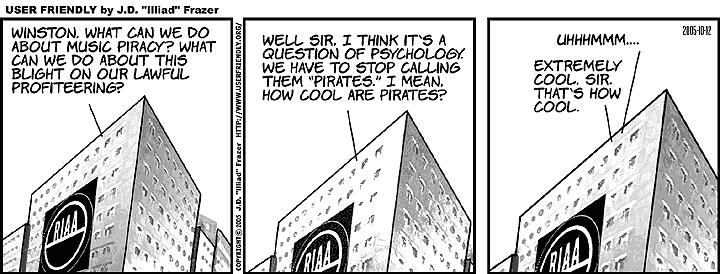
\includegraphics[width=\linewidth]
	  {bilder/comics/uf008412.png}    \end{center}
	  \begin{multicols}{2}

%%% Local Variables: 
%%% mode: latex
%%% TeX-master: "../../1-te"
%%% End: 
